\section{MUMPS: Process Pinning}
\label{subseq:mm-mumps-process-pinning}

Due to intensive and complex manipulations with frontal and and contribution matrices, we can assume that MUMPS belongs to memory bound applications. In this case memory access can be a bottleneck for the library. A common way to slightly improve efficiency of memory bound applications running on distributed memory machines, for example GMRES, is to distribute processes equally among sockets of  a node.\\


However, because MUMPS uses both task and data parallelism as well as a complex hybrid, both static and dynamic, task scheduling, it becomes difficult to decide which pinning strategy is better in terms of parallel performance i.e. \textit{close} or \textit{spread}, described in section \ref{subseq:matrix-sets-and-hardware}.\\


To find out, a couple of tests were prepared and ran with both GRS and SuiteSparse matrix sets. MUMPS library was downloaded, configured and compiled within PETSc environment with the default MUMPS settings. The tests were conducted on HW1  machine using only flat-MPI mode i.e. 1 thread per MPI process. Some results are shown in figure \ref{fig:mumps-close-vs-spread} and in appendix BRA-BRA where we measured time spent on all three phases i.e. analysis, factorization and solution.\\


\figpointer{\ref{fig:mumps-close-vs-spread}}
\begin{figure}
\centering
	\begin{tabular}{cc}
		\subfloat[k3-18]{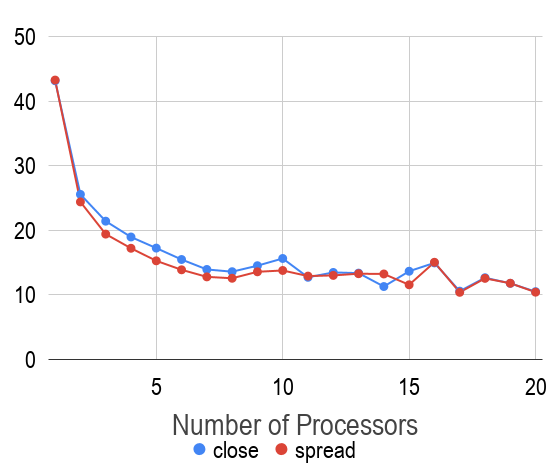
\includegraphics[width=0.45\textwidth]{figures/chapter-2/spread-vs-close/k3-18.png}} &
		\subfloat[cube-645]{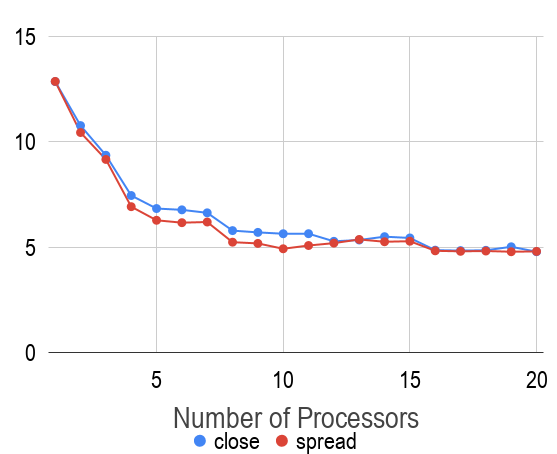
\includegraphics[width=0.45\textwidth]{figures/chapter-2/spread-vs-close/cube-645.png}} \\
		\subfloat[CurlCurl\_3]{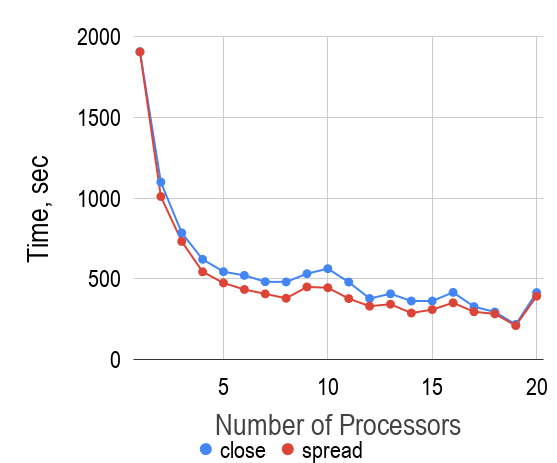
\includegraphics[width=0.45\textwidth]{figures/chapter-2/spread-vs-close/CurlCurl_3.png}} &
		\subfloat[memchip]{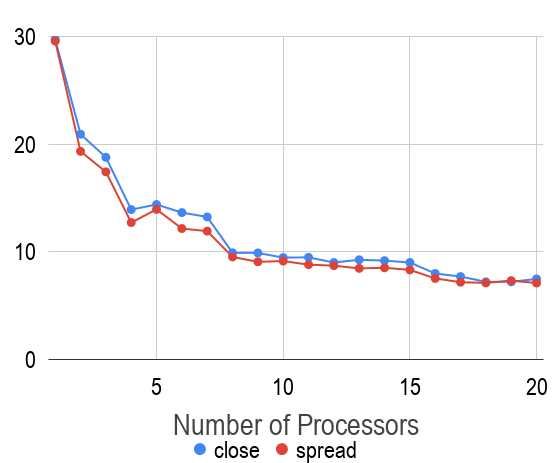
\includegraphics[width=0.45\textwidth]{figures/chapter-2/spread-vs-close/memchip.png}} \\
	\end{tabular}
	\caption{Comparison of \textit{close} and \textit{spread} pinning strategies}
	\label{fig:mumps-close-vs-spread}
\end{figure}


The tests revealed that \textit{spread}-pinning works better and allows to reduce run-time by approximately 5.5\% in average in contrast to the \textit{close} strategy. As expected, the points with 1 and 20 MPI processes show the same performance because they basically represent the same process distribution. Additionally, almost 13.5\% improvement can be observed around the saturation point in case of \textit{spread} strategy application.\\

Taken into consideration test results, \textit{spread}-pinning has been chosen for the rest of the study. Such process distribution can be easily achieved by means of some advanced OpenMPI options, for example \textit{--map-by}, as following:. \\

\begin{lstlisting}[language=bash, caption={An example of \textit{spread}-pinning with using OpenMPI options in case of a flat-MPI run}, frame=single, label={lst:iterative-refinement}]
mpiexec --map-by socket -n $num_proc $executable_name $parameters
\end{lstlisting}
